\chapter{Travessia de Grafos}

Este capítulo discute dois algoritmos fundamentais de grafos: busca em profundidade e busca em largura. Ambos os algoritmos recebem um nó inicial no grafo e visitam todos os nós que podem ser alcançados a partir do nó inicial. A diferença entre os algoritmos está na ordem em que eles visitam os nós.

\section{Busca em Profundidade}

\index{busca em profundidade}

\key{Busca em profundidade} (DFS) é uma técnica simples de travessia de grafos. O algoritmo começa em um nó inicial e prossegue para todos os outros nós que são alcançáveis a partir do nó inicial usando as arestas do grafo.

A busca em profundidade sempre segue um único caminho no grafo enquanto encontra novos nós. Depois disso, ele retorna aos nós anteriores e começa a explorar outras partes do grafo. O algoritmo mantém o controle dos nós visitados, para que processe cada nó apenas uma vez.

\subsubsection*{Exemplo}

Vamos considerar como a busca em profundidade processa o seguinte grafo:

\begin{center}
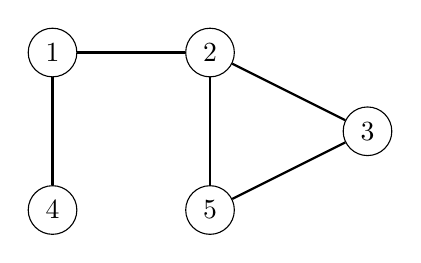
\begin{tikzpicture}
\node[draw, circle] (1) at (1,5) {$1$};
\node[draw, circle] (2) at (3,5) {$2$};
\node[draw, circle] (3) at (5,4) {$3$};
\node[draw, circle] (4) at (1,3) {$4$};
\node[draw, circle] (5) at (3,3) {$5$};

\path[draw,thick,-] (1) -- (2);
\path[draw,thick,-] (2) -- (3);
\path[draw,thick,-] (1) -- (4);
\path[draw,thick,-] (3) -- (5);
\path[draw,thick,-] (2) -- (5);
\end{tikzpicture}
\end{center}

Podemos começar a busca em qualquer nó do grafo; agora vamos começar a busca no nó 1.

A busca primeiro prossegue para o nó 2:

\begin{center}
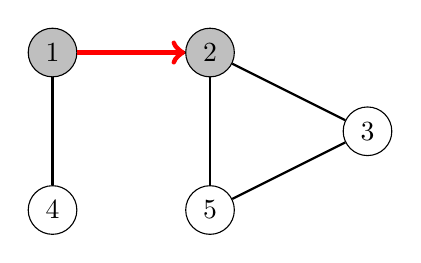
\begin{tikzpicture}
\node[draw, circle,fill=lightgray] (1) at (1,5) {$1$};
\node[draw, circle,fill=lightgray] (2) at (3,5) {$2$};
\node[draw, circle] (3) at (5,4) {$3$};
\node[draw, circle] (4) at (1,3) {$4$};
\node[draw, circle] (5) at (3,3) {$5$};

\path[draw,thick,-] (1) -- (2);
\path[draw,thick,-] (2) -- (3);
\path[draw,thick,-] (1) -- (4);
\path[draw,thick,-] (3) -- (5);
\path[draw,thick,-] (2) -- (5);

\path[draw=red,thick,->,line width=2pt] (1) -- (2);
\end{tikzpicture}
\end{center}

Depois disso, os nós 3 e 5 serão visitados:

\begin{center}
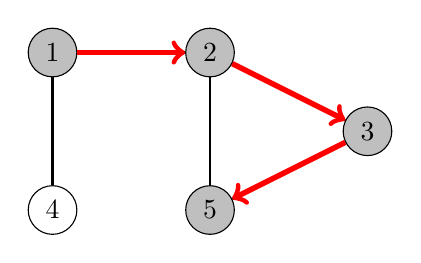
\begin{tikzpicture}
\node[draw, circle,fill=lightgray] (1) at (1,5) {$1$};
\node[draw, circle,fill=lightgray] (2) at (3,5) {$2$};
\node[draw, circle,fill=lightgray] (3) at (5,4) {$3$};
\node[draw, circle] (4) at (1,3) {$4$};
\node[draw, circle,fill=lightgray] (5) at (3,3) {$5$};

\path[draw,thick,-] (1) -- (2);
\path[draw,thick,-] (2) -- (3);
\path[draw,thick,-] (1) -- (4);
\path[draw,thick,-] (3) -- (5);
\path[draw,thick,-] (2) -- (5);

\path[draw=red,thick,->,line width=2pt] (1) -- (2);
\path[draw=red,thick,->,line width=2pt] (2) -- (3);
\path[draw=red,thick,->,line width=2pt] (3) -- (5);
\end{tikzpicture}
\end{center}

Os vizinhos do nó 5 são 2 e 3, mas a busca já visitou ambos, então é hora de retornar aos nós anteriores. Os vizinhos dos nós 3 e 2 também já foram visitados, então passamos do nó 1 para o nó 4:

\begin{center}
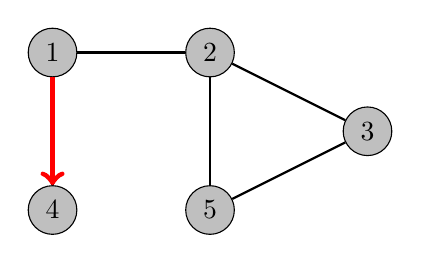
\begin{tikzpicture}
\node[draw, circle,fill=lightgray] (1) at (1,5) {$1$};
\node[draw, circle,fill=lightgray] (2) at (3,5) {$2$};
\node[draw, circle,fill=lightgray] (3) at (5,4) {$3$};
\node[draw, circle,fill=lightgray] (4) at (1,3) {$4$};
\node[draw, circle,fill=lightgray] (5) at (3,3) {$5$};

\path[draw,thick,-] (1) -- (2);
\path[draw,thick,-] (2) -- (3);
\path[draw,thick,-] (1) -- (4);
\path[draw,thick,-] (3) -- (5);
\path[draw,thick,-] (2) -- (5);

\path[draw=red,thick,->,line width=2pt] (1) -- (4);
\end{tikzpicture}
\end{center}

Depois disso, a busca termina porque visitou todos os nós.

A complexidade de tempo da busca em profundidade é $O(n+m)$ onde $n$ é o número de nós e $m$ é o número de arestas, porque o algoritmo processa cada nó e aresta uma vez.

\subsubsection*{Implementação}

A busca em profundidade pode ser convenientemente implementada usando recursão. A seguinte função \texttt{dfs} inicia uma busca em profundidade em um determinado nó. A função assume que o grafo é armazenado como listas de adjacência em um array:

\begin{lstlisting}
vector<int> adj[N];
\end{lstlisting}

e também mantém um array:

\begin{lstlisting}
bool visited[N];
\end{lstlisting}

que mantém o controle dos nós visitados. Inicialmente, cada valor do array é \texttt{false}, e quando a busca chega ao nó $s$, o valor de \texttt{visited}[$s$] se torna \texttt{true}. A função pode ser implementada da seguinte forma:

\begin{lstlisting}
void dfs(int s) {
    if (visited[s]) return;
    visited[s] = true;
    // processa o no s
    for (auto u: adj[s]) {
        dfs(u);
    }
}
\end{lstlisting}

\section{Busca em Largura}

\index{busca em largura}

\key{Busca em largura} (BFS) visita os nós em ordem crescente de sua distância do nó inicial. Assim, podemos calcular a distância do nó inicial a todos os outros nós usando a busca em largura. No entanto, a busca em largura é mais difícil de implementar do que a busca em profundidade.

A busca em largura percorre os nós um nível após o outro. Primeiro, a busca explora os nós cuja distância do nó inicial é 1, depois os nós cuja distância é 2 e assim por diante. Este processo continua até que todos os nós tenham sido visitados.

\subsubsection*{Exemplo}

Vamos considerar como a busca em largura processa o seguinte grafo:

\begin{center}
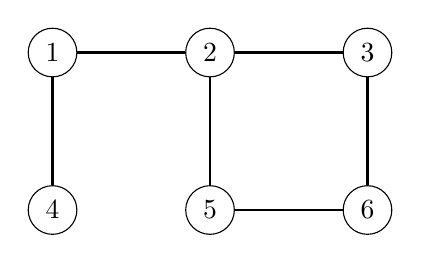
\begin{tikzpicture}
\node[draw, circle] (1) at (1,5) {$1$};
\node[draw, circle] (2) at (3,5) {$2$};
\node[draw, circle] (3) at (5,5) {$3$};
\node[draw, circle] (4) at (1,3) {$4$};
\node[draw, circle] (5) at (3,3) {$5$};
\node[draw, circle] (6) at (5,3) {$6$};

\path[draw,thick,-] (1) -- (2);
\path[draw,thick,-] (2) -- (3);
\path[draw,thick,-] (1) -- (4);
\path[draw,thick,-] (3) -- (6);
\path[draw,thick,-] (2) -- (5);
\path[draw,thick,-] (5) -- (6);
\end{tikzpicture}
\end{center}

Suponha que a busca comece no nó 1. Primeiro, processamos todos os nós que podem ser alcançados a partir do nó 1 usando uma única aresta:

\begin{center}
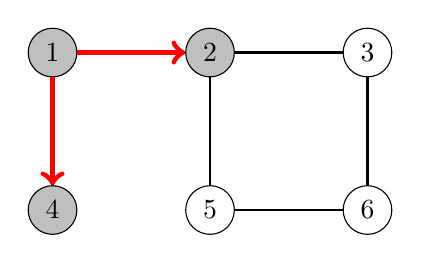
\begin{tikzpicture}
\node[draw, circle,fill=lightgray] (1) at (1,5) {$1$};
\node[draw, circle,fill=lightgray] (2) at (3,5) {$2$};
\node[draw, circle] (3) at (5,5) {$3$};
\node[draw, circle,fill=lightgray] (4) at (1,3) {$4$};
\node[draw, circle] (5) at (3,3) {$5$};
\node[draw, circle] (6) at (5,3) {$6$};

\path[draw,thick,-] (1) -- (2);
\path[draw,thick,-] (2) -- (3);
\path[draw,thick,-] (1) -- (4);
\path[draw,thick,-] (3) -- (6);
\path[draw,thick,-] (2) -- (5);
\path[draw,thick,-] (5) -- (6);

\path[draw,thick,-] (1) -- (2);
\path[draw,thick,-] (2) -- (3);
\path[draw,thick,-] (1) -- (4);
\path[draw,thick,-] (2) -- (5);

\path[draw=red,thick,->,line width=2pt] (1) -- (2);
\path[draw=red,thick,->,line width=2pt] (1) -- (4);
\end{tikzpicture}
\end{center}

Depois disso, prosseguimos para os nós 3 e 5:

\begin{center}
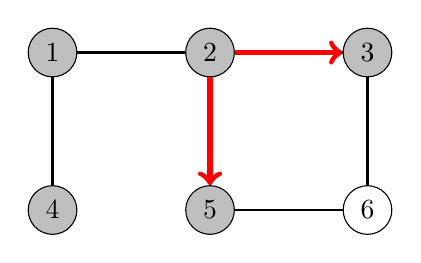
\begin{tikzpicture}
\node[draw, circle,fill=lightgray] (1) at (1,5) {$1$};
\node[draw, circle,fill=lightgray] (2) at (3,5) {$2$};
\node[draw, circle,fill=lightgray] (3) at (5,5) {$3$};
\node[draw, circle,fill=lightgray] (4) at (1,3) {$4$};
\node[draw, circle,fill=lightgray] (5) at (3,3) {$5$};
\node[draw, circle] (6) at (5,3) {$6$};

\path[draw,thick,-] (1) -- (2);
\path[draw,thick,-] (2) -- (3);
\path[draw,thick,-] (1) -- (4);
\path[draw,thick,-] (3) -- (6);
\path[draw,thick,-] (2) -- (5);
\path[draw,thick,-] (5) -- (6);

\path[draw,thick,-] (1) -- (2);
\path[draw,thick,-] (2) -- (3);
\path[draw,thick,-] (1) -- (4);
\path[draw,thick,-] (2) -- (5);

\path[draw=red,thick,->,line width=2pt] (2) -- (3);
\path[draw=red,thick,->,line width=2pt] (2) -- (5);
\end{tikzpicture}
\end{center}

Finalmente, visitamos o nó 6:

\begin{center}
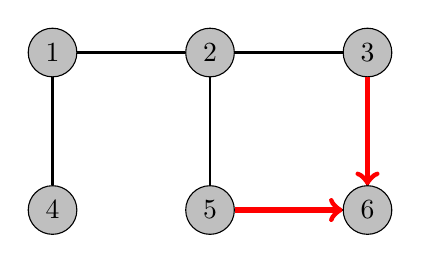
\begin{tikzpicture}
\node[draw, circle,fill=lightgray] (1) at (1,5) {$1$};
\node[draw, circle,fill=lightgray] (2) at (3,5) {$2$};
\node[draw, circle,fill=lightgray] (3) at (5,5) {$3$};
\node[draw, circle,fill=lightgray] (4) at (1,3) {$4$};
\node[draw, circle,fill=lightgray] (5) at (3,3) {$5$};
\node[draw, circle,fill=lightgray] (6) at (5,3) {$6$};

\path[draw,thick,-] (1) -- (2);
\path[draw,thick,-] (2) -- (3);
\path[draw,thick,-] (1) -- (4);
\path[draw,thick,-] (3) -- (6);
\path[draw,thick,-] (2) -- (5);
\path[draw,thick,-] (5) -- (6);

\path[draw,thick,-] (1) -- (2);
\path[draw,thick,-] (2) -- (3);
\path[draw,thick,-] (1) -- (4);
\path[draw,thick,-] (2) -- (5);

\path[draw=red,thick,->,line width=2pt] (3) -- (6);
\path[draw=red,thick,->,line width=2pt] (5) -- (6);
\end{tikzpicture}
\end{center}

Agora, calculamos as distâncias do nó inicial a todos os nós do grafo. As distâncias são as seguintes:

\begin{tabular}{ll}
\\
nó & distância \\
\hline
1 & 0 \\
2 & 1 \\
3 & 2 \\
4 & 1 \\
5 & 2 \\
6 & 3 \\
\\
\end{tabular}

Como na busca em profundidade, a complexidade de tempo da busca em largura é $O(n+m)$, onde $n$ é o número de nós e $m$ é o número de arestas.

\subsubsection*{Implementação}

A busca em largura é mais difícil de implementar do que a busca em profundidade, porque o algoritmo visita nós em diferentes partes do grafo. Uma implementação típica é baseada em uma fila que contém nós. A cada etapa, o próximo nó na fila será processado.

O código a seguir assume que o grafo é armazenado como listas de adjacência e mantém as seguintes estruturas de dados:

\begin{lstlisting}
queue<int> q;
bool visited[N];
int distance[N];
\end{lstlisting}

A fila \texttt{q} contém nós a serem processados em ordem crescente de sua distância. Novos nós são sempre adicionados ao final da fila, e o nó no início da fila é o próximo nó a ser processado. O array \texttt{visited} indica quais nós a busca já visitou e o array \texttt{distance} conterá as distâncias do nó inicial a todos os nós do grafo.

A busca pode ser implementada da seguinte forma, começando no nó $x$:

\begin{lstlisting}
visited[x] = true;
distance[x] = 0;
q.push(x);
while (!q.empty()) {
    int s = q.front(); q.pop();
    // processa o no s
    for (auto u : adj[s]) {
        if (visited[u]) continue;
        visited[u] = true;
        distance[u] = distance[s]+1;
        q.push(u);
    }
}
\end{lstlisting}

\section{Aplicações}

Usando os algoritmos de travessia de grafos, podemos verificar muitas propriedades dos grafos. Normalmente, tanto a busca em profundidade quanto a busca em largura podem ser usadas, mas na prática, a busca em profundidade é uma escolha melhor, porque é mais fácil de implementar. Nas seguintes aplicações, assumiremos que o grafo é não direcionado.

\subsubsection{Verificação de Conectividade}

\index{grafo conectado}

Um grafo é conectado se houver um caminho entre quaisquer dois nós do grafo. Assim, podemos verificar se um grafo é conectado começando em um nó arbitrário e descobrindo se podemos alcançar todos os outros nós.

Por exemplo, no grafo:

\begin{center}
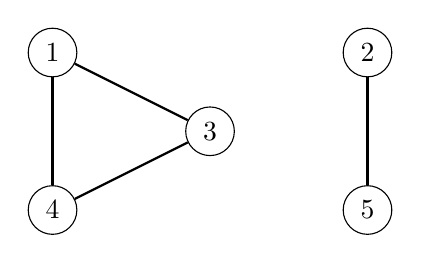
\begin{tikzpicture}
\node[draw, circle] (2) at (7,5) {$2$};
\node[draw, circle] (1) at (3,5) {$1$};
\node[draw, circle] (3) at (5,4) {$3$};
\node[draw, circle] (5) at (7,3) {$5$};
\node[draw, circle] (4) at (3,3) {$4$};

\path[draw,thick,-] (1) -- (3);
\path[draw,thick,-] (1) -- (4);
\path[draw,thick,-] (3) -- (4);
\path[draw,thick,-] (2) -- (5);
\end{tikzpicture}
\end{center}

uma busca em profundidade a partir do nó $1$ visita os seguintes nós:

\begin{center}
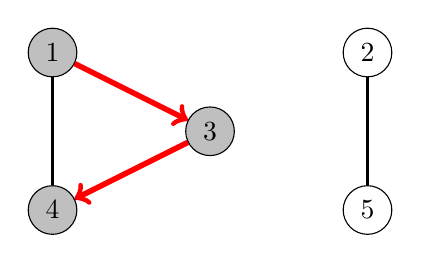
\begin{tikzpicture}
\node[draw, circle] (2) at (7,5) {$2$};
\node[draw, circle,fill=lightgray] (1) at (3,5) {$1$};
\node[draw, circle,fill=lightgray] (3) at (5,4) {$3$};
\node[draw, circle] (5) at (7,3) {$5$};
\node[draw, circle,fill=lightgray] (4) at (3,3) {$4$};

\path[draw,thick,-] (1) -- (3);
\path[draw,thick,-] (1) -- (4);
\path[draw,thick,-] (3) -- (4);
\path[draw,thick,-] (2) -- (5);

\path[draw=red,thick,->,line width=2pt] (1) -- (3);
\path[draw=red,thick,->,line width=2pt] (3) -- (4);

\end{tikzpicture}
\end{center}

Como a busca não visitou todos os nós, podemos concluir que o grafo não é conectado. De forma semelhante, também podemos encontrar todos os componentes conectados de um grafo iterando pelos nós e sempre iniciando uma nova busca em profundidade se o nó atual ainda não pertence a nenhum componente.

\subsubsection{Encontrando Ciclos}

\index{ciclo}

Um grafo contém um ciclo se, durante uma travessia de grafo, encontrarmos um nó cujo vizinho (diferente do nó anterior no caminho atual) já foi visitado. Por exemplo, o grafo:

\begin{center}
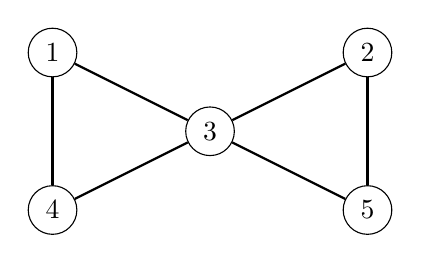
\begin{tikzpicture}
\node[draw, circle] (2) at (7,5) {$2$};
\node[draw, circle] (1) at (3,5) {$1$};
\node[draw, circle] (3) at (5,4) {$3$};
\node[draw, circle] (5) at (7,3) {$5$};
\node[draw, circle] (4) at (3,3) {$4$};

\path[draw,thick,-] (1) -- (3);
\path[draw,thick,-] (1) -- (4);
\path[draw,thick,-] (3) -- (4);
\path[draw,thick,-] (2) -- (5);
\path[draw,thick,-] (2) -- (3);
\path[draw,thick,-] (3) -- (5);
\end{tikzpicture}
\end{center}

contém dois ciclos e podemos encontrar um deles da seguinte forma:

\begin{center}
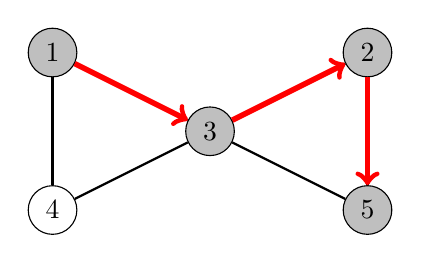
\begin{tikzpicture}
\node[draw, circle,fill=lightgray] (2) at (7,5) {$2$};
\node[draw, circle,fill=lightgray] (1) at (3,5) {$1$};
\node[draw, circle,fill=lightgray] (3) at (5,4) {$3$};
\node[draw, circle,fill=lightgray] (5) at (7,3) {$5$};
\node[draw, circle] (4) at (3,3) {$4$};

\path[draw,thick,-] (1) -- (3);
\path[draw,thick,-] (1) -- (4);
\path[draw,thick,-] (3) -- (4);
\path[draw,thick,-] (2) -- (5);
\path[draw,thick,-] (2) -- (3);
\path[draw,thick,-] (3) -- (5);

\path[draw=red,thick,->,line width=2pt] (1) -- (3);
\path[draw=red,thick,->,line width=2pt] (3) -- (2);
\path[draw=red,thick,->,line width=2pt] (2) -- (5);

\end{tikzpicture}
\end{center}

Depois de passar do nó 2 para o nó 5, notamos que o vizinho 3 do nó 5 já foi visitado. Assim, o grafo contém um ciclo que passa pelo nó 3, por exemplo, $3 \rightarrow 2 \rightarrow 5 \rightarrow 3$.

Outra forma de descobrir se um grafo contém um ciclo é simplesmente calcular o número de nós e arestas em cada componente. Se um componente contém $c$ nós e nenhum ciclo, ele deve conter exatamente $c-1$ arestas (portanto, deve ser uma árvore). Se houver $c$ ou mais arestas, o componente certamente contém um ciclo.

\subsubsection{Verificação de Bipartição}

\index{grafo bipartido}

Um grafo é bipartido se seus nós podem ser coloridos usando duas cores, de modo que não haja nós adjacentes com a mesma cor. É surpreendentemente fácil verificar se um grafo é bipartido usando algoritmos de travessia de grafo.

A ideia é colorir o nó inicial de azul, todos os seus vizinhos de vermelho, todos os seus vizinhos de azul e assim por diante. Se em algum ponto da busca notarmos que dois nós adjacentes têm a mesma cor, isso significa que o grafo não é bipartido. Caso contrário, o grafo é bipartido e uma coloração foi encontrada.

Por exemplo, o grafo:

\begin{center}
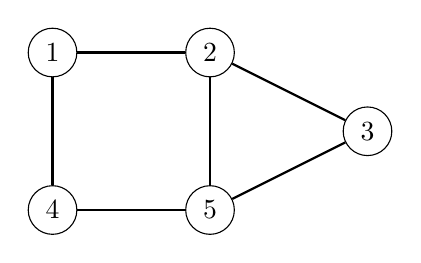
\begin{tikzpicture}
\node[draw, circle] (2) at (5,5) {$2$};
\node[draw, circle] (1) at (3,5) {$1$};
\node[draw, circle] (3) at (7,4) {$3$};
\node[draw, circle] (5) at (5,3) {$5$};
\node[draw, circle] (4) at (3,3) {$4$};

\path[draw,thick,-] (1) -- (2);
\path[draw,thick,-] (2) -- (5);
\path[draw,thick,-] (5) -- (4);
\path[draw,thick,-] (4) -- (1);
\path[draw,thick,-] (2) -- (3);
\path[draw,thick,-] (5) -- (3);
\end{tikzpicture}
\end{center}

não é bipartido, porque uma busca a partir do nó 1 prossegue da seguinte forma:

\begin{center}
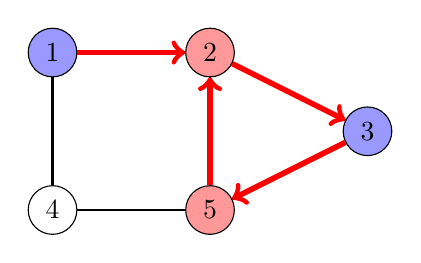
\begin{tikzpicture}
\node[draw, circle,fill=red!40] (2) at (5,5) {$2$};
\node[draw, circle,fill=blue!40] (1) at (3,5) {$1$};
\node[draw, circle,fill=blue!40] (3) at (7,4) {$3$};
\node[draw, circle,fill=red!40] (5) at (5,3) {$5$};
\node[draw, circle] (4) at (3,3) {$4$};

\path[draw,thick,-] (1) -- (2);
\path[draw,thick,-] (2) -- (5);
\path[draw,thick,-] (5) -- (4);
\path[draw,thick,-] (4) -- (1);
\path[draw,thick,-] (2) -- (3);
\path[draw,thick,-] (5) -- (3);

\path[draw=red,thick,->,line width=2pt] (1) -- (2);
\path[draw=red,thick,->,line width=2pt] (2) -- (3);
\path[draw=red,thick,->,line width=2pt] (3) -- (5);
\path[draw=red,thick,->,line width=2pt] (5) -- (2);
\end{tikzpicture}
\end{center}

Notamos que a cor de ambos os nós 2 e 5 é vermelha, sendo que eles são nós adjacentes no grafo. Assim, o grafo não é bipartido.

Este algoritmo sempre funciona, porque quando há apenas duas cores disponíveis, a cor do nó inicial em um componente determina as cores de todos os outros nós no componente. Não faz diferença se o nó inicial é vermelho ou azul.

Observe que, no caso geral, é difícil descobrir se os nós em um grafo podem ser coloridos usando $k$ cores para que nenhum nó adjacente tenha a mesma cor. Mesmo quando $k=3$, nenhum algoritmo eficiente é conhecido e o problema é NP-difícil.
